\section{Diskrete Zufallsvariablen und Verteilungen}
In diesem Kapitel ist $\Omega \neq \emptyset$ abzählbar oder endlich und $\mathcal{F} =  2^\Omega$ die Potenzmenge von $\Omega$, und damit das Wahrscheinlichkeitsmass $P$ gegeben durch seine Gewichte $p_i = P[\omega_i]$ für alle $i$.

\subsection{Grundbegriffe}
\begin{definition}[\textbf{diskrete Zufallsvariable}]
Eine \textit{reellwertige diskrete Zufallsvariable} auf $\Omega$ ist eine Funktion $X:\Omega \to \R$ mit abzählbarem Wertebereich $\mathcal{W}(X) = \{x_1,\dots,x_n\}$.
\begin{itemize}
\item die \textit{Verteilungsfunktion} von $X$ ist die Abbildung $F_X : \R \to [0,1]$ und ist definiert durch
$$ t \mapsto F_X(t) := P[X \leq t] := P[\{\omega \with X(\omega) \leq t\}]$$
\item die \textit{diskrete Dichte} von $X$ ist die Funktion $p_X : \mathcal{W}(X) \to [0,1]$ und ist definiert durch 
$$ p_X(x_k) := P[X = x_k] = P[\{\omega \with X(\omega) = x_k\}] \quad \quad \mbox{ für } k =1,2$$
\end{itemize}
\end{definition}
In unserem Fall mit $\Omega$ abzählbar und $\mathcal{F} = 2^\Omega$ ist \underline{jede Funktion} $X:\Omega \to \R$ eine Zufallsvariable. Sind $\Omega, \mathcal{F}$ allgemeiner, dann muss die obige Definition der Verteilung so angepasst werden, dass die Menge $\{X \leq t\}$ ein beobachtbares Ereignis für jedes $t$ ist, also in $\mathcal{F}$ ist. Das bedeutet, dass die Funktion $X$ im allgemeinen Fall $\mathcal{F}$-messbar sein muss.

\begin{definition}[\textbf{Indikatorfunktion}]
Für jede Teilmenge $A \subseteq \Omega$ ist die \textit{Indikatorfunktion} $I_A$ von $A$ definiert durch 
$$ I_A(\omega) := \begin{cases} 1 & \mbox{falls } \omega \in A \\ 0 & \mbox{falls } \omega \in A^\complement \end{cases}$$
\end{definition}
In unserem Fall ist $I_A$ für jedes $A \subseteq \Omega$ eine Zufallsvariable.

\subsubsection*{Eigenschaften der Dichte und Verteilungsfunktion}
\begin{itemize}
\item die Verteilungsfunktion $F_X$ ist vollständig durch die Dichte $p_X$ festgelegt, nämlich: $F_X(t) = P[X \leq t] = \sum_{k \mbox{ mit } x_k \leq t} \{X = x_k\}$
\item für jedes $x_k \in \mathcal{W}(X)$ gilt $0 \leq p_X(x_k) \leq 1$ und $\sum_{x_k \in \mathcal{W}(X)} p_X(x_k) = 1$.
\item ist $\mathcal{W}$ nichtleer und abzählbar und $f:\mathcal{W}\to \R$ eine Funktion zwischen 0 und 1 für jedes $w_k \in \mathcal{W}$ mit $\sum_{w_k \in \mathcal{W}} f(w_k) = 1$, dann kann man einen Wahrscheinlichkeitsraum $(\Omega, \mathcal{F}, P)$ und darauf eine Zufallsvariable $X$ konstruieren, deren Gewichtsfunktion gerade die Funktion $f$ ist. Dazu genügt bspw. $\Omega := \mathcal{W}$, $\mathcal{F} := 2^\Omega$ und $X(\omega) = \omega$.
\item Die Verteilung beschreibt das stochastische Verhalten einer Zufallsvariable. Das ist dasjenige Wahrscheinlichkeitsmass $\mu_X$ auf $\R$, das durch $\mu_X(B) := P[X \in B]$ definiert ist. Ist $X$ diskrete Zufallsvariable $\implies \mu_X$ heisst \textit{diskrete Verteilung}. Damit kann man die Verteilung $\mu_X$ und die Gewichtsfunktion $p_X$ direkt miteinander identifizieren: der einzige Unterschied besteht darin, dass $\mu_X$ als Argumente \textit{Teilmengen} von $\mathcal{W(X)}$ hat, $p_X$ hingegen \textit{Elemente} von $\mathcal{W}(X)$. Folgende Formel beschreibt ihren Zusammenhang:
$$ \mu_X(B) = P[X \in B] = \sum_{x_k \in B} p_X(x_k) \quad \quad \mbox{ für } B\subseteq \mathcal{W}(X)$$
\end{itemize}


\subsection{Erwartungswerte}
\begin{definition}[\textbf{Erwartungswert}]
Sei $X$ eine diskrete Zufallsvariable mit Gewichtsfunktion $p_X(x)$, dann ist der \textit{Erwartungswert} definiert als
$$ \E[X] := \sum_{x_k \in \mathcal{W}(X)} x_K \cdot p_X(x_k)$$
sofern diese Reihe absolut konvergiert. Ansonsten existiert der Erwartungswert nicht.
\end{definition}
Man kann den Erwartungswert auch als Summe über $\Omega$ schreiben, falls er exisitert, denn dann gilt:
$$ \E[X] = \sum_{\omega_i \in \Omega} X(\omega_i) P[\{\omega_i\}] = \sum_{\omega_i \in \Omega} p_i X(\omega_i)$$
(eine weitere Umformung existiert im Skript, Seite 43)

\begin{satz}[\textbf{Erwartungswert von Funktionen von ZV}]
Sei $X$ eine diskrete Zufallsvariable mit Gewichtsfunktion $p_X(x)$ und $Y = g(X)$ für eine Funktion $g:\R \to \R$. Dann gilt
$$ \E[Y] = \E[g(X)] = \sum_{x_k \in \mathcal{W}(X)} g(x_k) \cdot p_X(x_k)$$
sofern die Reihe absolut konvergiert.
\end{satz}
Damit genügt es, die Verteilung von $X$ zu kennen, man muss nicht extra die Verteilung von $Y$ zuerst bestimmen, um den Erwartungswert von $Y$ zu berechnen.

\begin{satz}[\textbf{Eigenschaften des Erwartungswerts}]
Seien $X,Y$ Zufallsvariablen mit existentem Erwartungswert. Dann gilt:
\begin{itemize}
\item[(i)] \textbf{Monotonie:} $X \leq Y \implies \E[X] \leq \E[Y]$ wobei dies bedeutet, dass $X(\omega) \leq Y(\omega)$ für alle $\omega$.
\item[(ii)] \textbf{Linearität:} für beliebige $a,b \in \R$ gilt: $\E[aX+b] = a\E[X] + b$
\item[(iii)] nimmt $X$ nur Werte aus $\N_0 = \{0,1,2,\dots\}$ annimmt, dann gilt:
$$ \E[X] = \sum_{j=1}^\infty P[X \geq j] = \sum_{l = 0}^\infty [P_X \geq l]$$
\end{itemize}
\end{satz}

\begin{definition}[\textbf{Varianz \& Standardabweichung}]
Sei $X$ eine diskrete ZV mit $\E[X^2] < \infty$\\ dann definieren wir die \textit{Varianz} von $X$ als
$$ \mbox{Var}[X] := \E\left[(X - \E[X])\right]$$ und die \textit{Standardabweichung} von $X$ als
$$ \sigma(X) = \mbox{sd}(X) := \sqrt{\mbox{Var}[X]}$$
Beides sind \textit{Streuungsmasse} für die Verteilung von $X$
\end{definition}

Schreiben wir $m_X := \E[X]$ und definieren die Funktion $g(x):= (x-m_X)^2$, dann erhalten wir
$$ \mbox{Var}[X] = \sum_{x_k \in \mathcal{W}(X)} (x_k - m_X)^2 \cdot p_X(x_K)$$

\begin{lemma}
Die Varianz von Zufallsvariablen hat folgende Eigenschaften:
\begin{itemize}
\item[(i)] Var$[X] = \E[X^2] - (\E[X])^2$
\item[(ii)] Var$[aX + b] = a^2 \cdot $Var$[X]$
\end{itemize}
\end{lemma}


\subsection{Gemeinsame Verteilungen \& Unabhängige Zufallsvariablen}
\begin{definition}[\textbf{Gemeinsame Verteilung \& Dichte}]
Seien $X_1,\dots, X_n$ Zufallsvariablen. Die \textit{gemeinsame Verteilungsfunktion} von $X_1,\dots,X_n$ ist die Abbildung $F:\R^n \to [0,1]$ definiert durch 
$$ (x_1,\dots,x_n) \mapsto F(x_1,\dots,x_n) := P[X_1 \leq x_1, \dots, X_n \leq x_n]$$
Sind $X_1, \dots, X_n$ diskrete Zufallsvariablen, so definiert man ihre \textit{gemeinsame Gewichtsfunktion} $p:\R^n \to [0,1]$ durch 
$$ p(x_1,\dots,x_n):= P[X_1 = x_1, \dots, X_n = x_n]$$.
Es ist klar, dass $p(x_1,\dots,x_n) = 0$ falls das Ereignis $(x_1, \dots, x_n)$ nicht im gemeinsamen Wertebereich liegt.
\end{definition}
Aus der gemeinsamen Gewichtsfunktion $p$ erhält man die gemeinsame Verteilungsfunktion:
$$ F(x_1, \dots, x_n) = \sum_{y_1 \leq x_1, \dots, y_n \leq x_n} p(y_1,\dots,y_n)$$

\begin{definition}[\textbf{Randverteilung}]
Sein $X,Y$ Zufallsvariablen mit der gemeinsamen Verteilungsfunktion $F$. Dann ist die \textit{Randverteilung} von $X$ gegeben durch
$$F_X:\R \to [0,1] \mbox{  mit  } x\mapsto F_X(x) := P[X \leq x] = P[X \leq x, Y < \infty] = \lim_{y\to \infty} F(x,y)$$
Sind $X,Y$ diskrete Zufallsvariablen mit $\mathcal{W}(Y) = \{y_1,y_2,\dots \}$ und gemeinsamer Gewichtsfunktion $p(x,y)$, so ist die \textit{Gewichtsfunktion der Randverteilung} von $X$ gegeben durch

\begin{align*}
	p_X: \mathcal{W}(X) \to [0,1] \mbox{  mit  } x \mapsto p_X(x) &= P[X=x] \\&= \sum_{y_j \in \mathcal{W}(Y)} P[X=x, Y = y_j] \\&= \sum_{y_j \in \mathcal{W}(Y)} p(x,y_j) \quad \mbox{ für } x\in \mathcal{W}(X)
\end{align*}
Analoge Aussagen gelten natürlich für $Y$.
\end{definition} 

Für Vektoren von diskreten Zufallsvariablen $(X_1, \dots, X_n)$ definiert man die Randverteilungen für jeden möglichen \textit{Teilvektor} von $(X_1,\dots, X_n)$. Es gibt also eindimensionale, aber auch multi-dimensionale Randverteilungen!\\

Bei zweidimensionalen diskreten Zufallsvariablen erhält man die Gewichtsfunktionen der Randverteilungen als Zeilen- bzw. Spaltensummen der gemeinsamen Gewichtsfunktionen, wie das folgende Bespiel illustriert:
\begin{center}
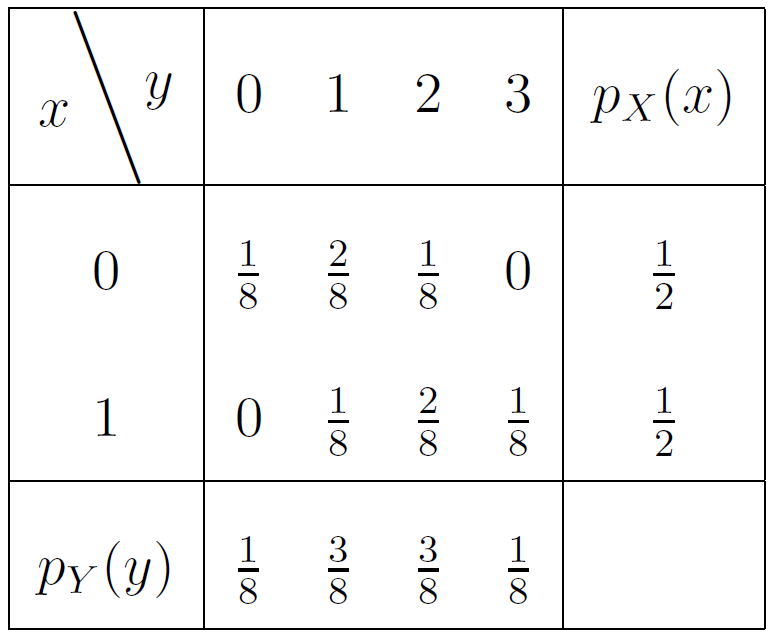
\includegraphics[scale=0.44]{randverteilung.png}
\end{center}
Aus den Randverteilungen kann man jedoch nicht ohne Weiteres die gemeinsame Verteilung herleiten, dazu fehlt Information über die \textit{Abhängigkeitsstruktur} der Zufallsvariable.

\begin{definition}[\textbf{Unabhängigkeit}]
Zufallsvariablen $X_1,\dots, X_n$ heissen \textit{unabhängig}, falls gilt
$$ F(x_1, \dots, x_n) = F_{X_1}(x_1) \cdots F_{X_n}(x_n)$$
\end{definition}
Folgendes Lemma gibt den Zusammenhang zu unabhängigen Ereignissen:
\begin{lemma}
Die diskreten Zufallsvariablen $X_1,\dots, X_n$ sind unabhängig\\ 
$\LLRA$ für beliebige Teilmengen $B_i \subseteq \mathcal{W}(X_i), i = 1\dots n$ sind die Ereignisse $A_i := \{X_i \in B_i\}$ für $i= 1\dots n$ unabhängig \\
$\LLRA$ für beliebige Teilmengen $B_i \subseteq \mathcal{W}(X_i), i = 1\dots n$ gilt:
$$ P[X_1 \in B_1, \dots, X_n \in B_n] = \prod_{i=1}^n P[X_i \in B_i]$$
\end{lemma}

\begin{satz}[\textbf{Funktionen auf Zufallsvariablen}]
Seien $X_1,\dots, X_n$ diskrete unabhängige Zufallsvariablen und $f_i :\R \to \R$ irgendwelche Funktionen. Sei weiter $Y_i := f_i(X_i)$ für $ 1 \leq 1 \leq n$. Dann sind die Zufallsvariablen $Y_1,\dots, Y_n$ ebenfalls unabhängig.
\end{satz}

\subsection{Funktionen von mehreren Zufallsvariablen}
Sind $X_1,\dots,X_n$ diskrete Zufallsvariablen, dann ist $Y = g(X_1,\dots,X_n)$ wieder eine Zufallsvariable für eine Funktion $g:\R^n \to \R$.

\begin{satz}
Seien $X_1,\dots,X_n$ diskrete Zufallsvariablen mit endlichen Erwartungswerten. Sei $Y = a + \sum_{i=0}^n  b_i X_i$ für Konstanten $a,b_i$. Dann gilt:
$$ \E[Y] = a + \sum_{i = 0}^n b_i \E[X_i]$$
\end{satz}

\begin{definition}[\textbf{Kovarianz}]
Seien $X,Y$ Zufallsvariablen auf einem Wahrscheinlichkeitsraum $(\Omega, \mathcal{F}, P)$ mit endlichen Erwartungswerten. Dann ist die \textit{Kovarianz} definiert als
$$ Cov(X,Y) := \E[(X-\E[X])(Y-\E[Y])] = \E[XY] - \E[X]\E[Y]$$
\end{definition}

\begin{definition}[\textbf{Korrelation}]
Die Korrelation von $X$ und $Y$ ist definiert durch
$$ \rho(X,Y) := \begin{cases} \frac{Cov(X,Y)}{\sigma(X)\sigma(Y)} & \mbox{falls } \sigma(X)\sigma(Y) > 0 \\ 0 & \mbox{sonst} \end{cases}$$
\end{definition}

\begin{satz}[\textbf{Wertebereich der Korrelation}]
Seien $X,Y$ wie in der Definition der Kovarianz, dann folgt aus der Cauchy-Schwarz Ungleichung, dass $|Cov(X,Y)| \leq \sigma(X)\sigma(Y)$, und damit folgt für die Korrelation
$$ -1 \leq \rho(X,Y) \leq 1$$
\end{satz}

Wir haben bereits gesehen, dass der Erwartungswert linear ist. Für die Varianz ist dies nicht ganz so einfach. Es gilt:

\begin{korollar}[\textbf{Summenformel für Varianzen}]
$$ \mbox{Var}\left[\sum_{i=1}^n X_i \right] = \sum_{i=1}^n \mbox{Var}[X_i] + 2 \cdot \sum_{i < j} Cov(X_i, X_j)$$
\end{korollar}
Ist $Cov(X,Y) = 0$, so nennt man $X$ und $Y$ \textbf{unkorreliert}. $\implies$ Linearität der Varianz gilt nur für unkorrelierte Zufallsvariablen. Für Produkte von Zufallsvariablen gilt:

\begin{satz}[\textbf{Produkte von Zufallsvariablen}]
Seien $X_1,\dots, X_n$  diskrete Zufallsvariablen mit endlichen Erwartungswerten. Falls $X_1,\dots,X_n$ unabhängig sind, dann gilt
$$\E\left[\prod_{i=1}^n X_i\right] = \prod_{i=1}^n \E[X_i]$$ Insbesondere sind $X_1,\dots,X_n$ paarweise unkorreliert und und daher gilt
$$ \mbox{Var}\left[\sum_{i=1}^n X_i\right] = \sum_{i=1}^n \mbox{Var}[X_i]$$ sofern die Varianzen existieren und endlich sind.
\end{satz}
\underline{Bemerkung:} Es gilt die Implikationskette: unabhängig $\implies$ paarweise unabhängig $\implies$ unkorreliert\\

\underline{Bemerkung:} Es gibt keine allgemeine Produktregel für Varianzen!

\subsubsection*{Faltung}
Seien $X,Y$ diskrete Zufallsvariablen mit gemeinsamer Gewichtsfunktion $p(x,y)$. Dann ist auch ihre Summe $Z:=X+Y$ diskret. Damit können wir die Gewichtsfunktion von $Z$ beschreiben durch
$$ p_Z(z) = P[Z=z] = \sum_{x_k \in \mathcal{W}(X)} P[X=x_k, Y = z-x_k] = \sum_{x_k \in \mathcal{W}(X)} p(x_k, z-x_k)$$ oder analog via Symmetrie $= \sum_{y_j\in\mathcal{W}(Y)} p(z-y_j, y_j)$. Dies ist ein völlig allgemeines Resultat. Sind nun $X$ und $Y$ unabhängig, dann gilt bekanntlich $p(x,y)= p_X(x) \cdot p_Y(y)$. Damit folgt die bekannte \textit{Faltung} der Gewichtsfunktionen $p_X$ und $p_Y$:
$$ p_Z(z) = \sum_{x_k \in \mathcal{W}(X)} p_X(x_k) \cdot p_Y(z-x_k) = \sum_{y_j \in \mathcal{W}(Y)} p_X(z-y_j) \cdot p_Y(y_j)$$ und schreiben dies kurz als $p_Z = p_X * p_Y = p_Y * p_X$.

\subsection{Bedingte Verteilungen}
Hier haben wir die gemeinsame Verteilung zweier Zufallsvariablen und wollen Informationen, die wir über eine der beiden Zufallsvariablen haben, ausnutzen um eine genauere Aussage über die andere Zufallsvariable zu machen.

\begin{definition}[\textbf{bedingte Gewichtsfunktion}]
$X,Y$ diskrete ZV mit gemeinsamer Gewichtsfunktion $p(x,y)$. Die \textit{bedingte Gewichtsfunktion} von $X$, gegeben dass $Y=y$, ist definiert als
$$ p_{X \with Y} (x \with y) := P[X=x \with Y=y] = \frac{P[X=x, Y = y]}{P[Y=y]} = \frac{p(x,y)}{p_Y(y)} $$
für $p_Y(y) >0$ und 0 sonst.
\end{definition}

\begin{lemma}[\textbf{Kriterium für Unabhängigkeit}]
Aus der Charakterisierung der Unabhängigkeit folgt sofort: \\
$X$ und $Y$ sind unabhängig $\LLRA$ für alle $y$ mit $p_Y(y)>0$ gilt: $p_{X \with Y} (x \with y) = p_X(x) \quad \forall x\in \mathcal{W}(X)$.
\end{lemma}
Eine symmetrische Aussage gilt natürlich, wenn $X$ und $Y$ vertauscht werden.\\

\underline{Bemerkung:} Man kann auch auf ein Ereignis bedingen, welches man dann mithilfe einer Indikatorvariable in eine Zufallsvariable verwandelt (siehe Beispiel Seite 64)
